% file: counting-sort-cycle-example.tex

\documentclass[tikz]{standalone}
\usetikzlibrary{decorations.pathreplacing, positioning, arrows.meta, shapes.multipart}

\newcommand{\red}[1]{\textcolor{red}{#1}}
\newcommand{\blue}[1]{\textcolor{blue}{#1}}
\newcommand{\purple}[1]{\textcolor{purple}{#1}}

\begin{document}
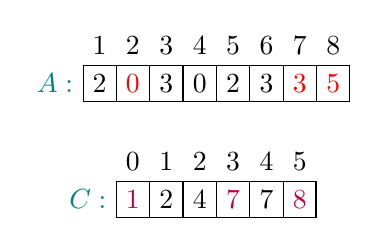
\begin{tikzpicture}[Array/.style = {rectangle split, rectangle split parts = #1, rectangle split horizontal, 
  	anchor = center}]
  % input A
  \node[Array = {8}, draw, label = {left: \textcolor{teal}{$A:$}}] (A) 
    {2\nodepart{two}\red{0}\nodepart{three}3\nodepart{four}0\nodepart{five}2\nodepart{six}3\nodepart{seven}\red{3}\nodepart{eight}\red{5}};
  \node[Array = {8}, above = 0.cm of A] (A-index) 
    {1\nodepart{two}2\nodepart{three}3\nodepart{four}4\nodepart{five}5\nodepart{six}6\nodepart{seven}7\nodepart{eight}8};

  % counting C'
  \node[Array = {6}, draw, below = 1.0cm of A, label = {left: \textcolor{teal}{$C:$}}] (C') 
    {\purple{1}\nodepart{two}2\nodepart{three}4\nodepart{four}\purple{7}\nodepart{five}7\nodepart{six}\purple{8}};
  \node[Array = {6}, above = 0.cm of C'] (C-index) 
    {0\nodepart{two}1\nodepart{three}2\nodepart{four}3\nodepart{five}4\nodepart{six}5};
\end{tikzpicture}
\end{document}

